\documentclass[9pt]{IEEEtran}

\usepackage[english]{babel}
\usepackage{graphicx}
\usepackage{epstopdf}
\usepackage{fancyhdr}
\usepackage{amsmath}
\usepackage{amsthm}
\usepackage{amssymb}
\usepackage{url}
\usepackage{array}
\usepackage{textcomp}
\usepackage{listings}
\usepackage{hyperref}
\usepackage{xcolor}
\usepackage{colortbl}
\usepackage{float}
\usepackage{gensymb}
\usepackage{longtable}
\usepackage{supertabular}
\usepackage{multicol}

\usepackage[utf8x]{inputenc}

\usepackage[T1]{fontenc}
\usepackage{lmodern}
\usepackage{multirow}
\input{glyphtounicode}
\pdfgentounicode=1

\graphicspath{{./figures/}}
\DeclareGraphicsExtensions{.pdf,.png,.jpg,.eps}

% correct bad hyphenation here
\hyphenation{op-tical net-works semi-conduc-tor trig-gs}

% ============================================================================================

\title{\vspace{0ex}
Programming part}


% ============================================================================================

\begin{document}

\maketitle

\section{Problems 3,4, and 5}
In this section we implemented gradient descent, Polyak gradient descent, 
Nesterov Gradient descent, AdaGrad gradient descent, the Newton method, 
the BFGS method and the L\_BFGS method. We tested all of the listed methods 
on three different functions and 2 different starting points(for each function).
For each function we tested which method performs best in 2,5,10 and 100 steps.
We also tested which performs best in 0.1, 1 and 2 seconds.

\subsection{Function 1}
The first funcion was given as:
\[
f_1(x) = (x_0 - x_2)^2 + (2x_1 + x_2)^2 + (4x_0 - 2x_1 + x_2)^2 + x_0 + x_1
\]
with the gradient of:
\[
\nabla f_1(x) =
\begin{bmatrix}
2(x_0 - x_2) + 8(4x_0 - 2x_1 + x_2) + 1 \\
4(2x_1 + x_2) - 4(4x_0 - 2x_1 + x_2) + 1 \\
6x_0 + 6x_2
\end{bmatrix}
\]
and the Hessian matrix:
\[
\nabla^2 f_1(x) =
\begin{bmatrix}
34 & -16 & 6 \\
-16 & 16 & 0 \\
6 & 0 & 6
\end{bmatrix}
\]
This function has a nice constant positive definite Hessian so none of the 
functions really have problems to converge to the minimum. Note that for all the functions 
we used a learning rate (for gradient descent methods) of 0.001, except for the AdaGrad where 
it was set to 1. We set the momentum coefficient to 0.5. The m in the L-BFGS method
was set to 10. We set our convergence 
condition to be where the difference in our positions is small enough. These conditions hold throughout all three 
functions.
\\ In Table~\ref{tab:f1} we 
can see the results when setting the methods to different amounts of maximum iterations. Note 
that S1 and S2 denote the different starting points. Also note that Max S denotes the maximum number 
of steps.
We can see that for this function the Newton and quasi-Newton methods converge very fast in 
comparison to the gradient descent methods, which is not suprising since this function is quadratic. 
Comparing just the gradient descent methods, we can see that AdaGrad is by far the best, followed by 
Polyak and Nesterov methods, and lastly the normal gradient descent which shows the slowest convergence.  
\\
We also tested the methods when limited to the specified time frames, however for this function 
all of the methods converged already in the smallest time frame. The results of the final 
convergence of methods is presented in Table~\ref{tab:f1_time}. We can see that all the methods 
converged to the same minimum however the Newton and quasi-Newton methods used considerabely less 
iterations to do so. Among the gradient descent methods, we can conclude the same as for the previous 
table.



\begin{table}[h!]
    \centering
    \begin{tabular}{|c|c|c|c|c|c|c|}
        \hline
        \multirow{2}{*}{\textbf{Method}} & \multirow{2}{*}{\textbf{Max S}} & \multicolumn{2}{c|}{\textbf{f1 Value}} & \multicolumn{2}{c|}{\textbf{Steps}} \\ \cline{3-4} \cline{5-6}
                                          &                                  & \textbf{S1} & \textbf{S2} & \textbf{S1} & \textbf{S2} \\ \hline
        \multirow{7}{*}{GD}              & 2  & -0.0039  & 10.2427  & 2  & 2 \\ \cline{2-6} 
                                       & 5  & -0.0096  & 9.2779   & 5  & 5 \\ \cline{2-6} 
                                       & 10 & -0.0185  & 8.0179   & 10 & 10 \\ \cline{2-6} 
                                       & 50 & -0.0713  & 3.7972   & 50 & 50 \\ \cline{2-6} 
                                       & 100& -0.1114  & 1.9365   & 100 & 100 \\ \hline
        \multirow{7}{*}{Polyak}       & 2  & -0.0049  & 10.0584  & 2  & 2 \\ \cline{2-6} 
                                       & 5  & -0.0153  & 8.3858   & 5  & 5 \\ \cline{2-6} 
                                       & 10 & -0.0317  & 6.4749   & 10 & 10 \\ \cline{2-6} 
                                       & 50 & -0.1109  & 1.9411   & 50 & 50 \\ \cline{2-6} 
                                       & 100& -0.1532  & 0.6071   & 100 & 100 \\ \hline
        \multirow{7}{*}{Nesterov}     & 2  & -0.0049  & 9.8163   & 2  & 2 \\ \cline{2-6} 
                                       & 5  & -0.0152  & 8.1940   & 5  & 5 \\ \cline{2-6} 
                                       & 10 & -0.0315  & 6.3939   & 10 & 10 \\ \cline{2-6} 
                                       & 50 & -0.1106  & 1.9378   & 50 & 50 \\ \cline{2-6} 
                                       & 100& -0.1530  & 0.6091   & 100 & 100 \\ \hline
        \multirow{7}{*}{AdaGrad}         & 2  & 24.5474  & 7.3378   & 2  & 2 \\ \cline{2-6} 
                                       & 5  & 0.7125   & 0.5004   & 5  & 5 \\ \cline{2-6} 
                                       & 10 & 0.0095   & -0.1905  & 10 & 10 \\ \cline{2-6} 
                                       & 50 & -0.1979  & -0.1979  & 50 & 50 \\ \cline{2-6} 
                                       & 100& -0.1979  & -0.1979  & 100 & 100 \\ \hline
        \multirow{7}{*}{Newton}          & 2  & -0.1979  & -0.1979  & 1  & 1 \\ \cline{2-6} 
                                       & 5  & -0.1979  & -0.1979  & 1  & 1 \\ \cline{2-6} 
                                       & 10 & -0.1979  & -0.1979  & 1  & 1 \\ \cline{2-6} 
                                       & 50 & -0.1979  & -0.1979  & 1  & 1 \\ \cline{2-6} 
                                       & 100& -0.1979  & -0.1979  & 1  & 1 \\ \hline
        \multirow{7}{*}{BFGS}            & 2  & -0.1114  & 5.0201   & 2  & 2 \\ \cline{2-6} 
                                       & 5  & -0.1566  & 0.6331   & 5  & 5 \\ \cline{2-6} 
                                       & 10 & -0.1597  & 0.5838   & 10 & 10 \\ \cline{2-6} 
                                       & 50 & -0.1979  & -0.1979  & 20 & 22 \\ \cline{2-6} 
                                       & 100& -0.1979  & -0.1979  & 20 & 22 \\ \hline
        \multirow{7}{*}{L-BFGS}          & 2  & 7.0000   & 6246.0000 & 2  & 2 \\ \cline{2-6} 
                                       & 5  & -0.1806  & 0.1495   & 5  & 5 \\ \cline{2-6} 
                                       & 10 & -0.1979  & -0.1979  & 8  & 10 \\ \cline{2-6} 
                                       & 50 & -0.1979  & -0.1979  & 8  & 11 \\ \cline{2-6} 
                                       & 100& -0.1979  & -0.1979  & 8  & 11 \\ \hline
    \end{tabular}
    \vspace{3pt}
    \caption{Performance of various optimization methods with different numbers of maximum steps and starting points for the first 
    function}
    \label{tab:f1}
\end{table}

\begin{table}[h!]
    \centering
    \begin{tabular}{|c|c|c|c|c|}
        \hline
        \textbf{Method} & \textbf{S1: f1} & \textbf{S1: Steps} & \textbf{S2: f1} & \textbf{S2: Steps} \\ \hline
        GD         & -0.1979  & 3142  & -0.1979  & 3611 \\ \hline
        Polyak     & -0.1979  & 1561  & -0.1979  & 1794 \\ \hline
        Nesterov   & -0.1979  & 1565  & -0.1979  & 1798 \\ \hline
        AdaGrad    & -0.1979  & 101   & -0.1979  & 79   \\ \hline
        Newton     & -0.1979  & 1     & -0.1979  & 1    \\ \hline
        Bfgs       & -0.1979  & 20    & -0.1979  & 22   \\ \hline
        L-Bfgs    & -0.1979  & 8     & -0.1979  & 11   \\ \hline
    \end{tabular}
    \vspace{3pt}
    \caption{Performance of various optimization methods with different starting points for the first function}
    \label{tab:f1_time}
\end{table}

\clearpage
\subsection{Function 2}
The second function was given as:
\[
f_2(x) = (x_1 - 1)^2 + (x_2 - 1)^2 + 100 \cdot (x_2 - x_1^2)^2 + 100 \cdot (x_3 - x_2^2)^2
\]
with the gradient:
% Gradient of f2
\[
\nabla f_2(x) = \begin{bmatrix}
    2(x_1 - 1) - 400x_1(x_2 - x_1^2) \\
    2(x_2 - 1) + 200(x_2 - x_1^2) - 400x_2(x_3 - x_2^2) \\
    100(x_3 - x_2^2)
\end{bmatrix}
\]
and the hessian matrix:
\[
H_f(x) = \begin{bmatrix}
    1200x_1^2 - 400x_2 + 2 & -400x_1 & 0 \\
    -400x_1 & 1200x_2^2 - 400x_3 + 202 & -400x_2 \\
    0 & -400x_2 & 200
\end{bmatrix}
\]
This function is not as simple as the previous one. In Table~\ref{tab:f2} we can see that all the methods, including 
the newton and the quasi-newton mtehods cannot converge even in 100 steps. In this case the performance of the 
 gradient descent methods are closer to the Newton and quasi-Newton methods.  

\begin{table}[h!]
    \centering
    \begin{tabular}{|p{1cm}|p{1cm}|p{1.7cm}|p{1.7cm}|p{0.5cm}|p{0.5cm}|}
        \hline
        \multirow{2}{*}{\textbf{Method}} & \multirow{2}{*}{\textbf{Max S}} & \multicolumn{2}{c|}{\textbf{f2 Value}} & \multicolumn{2}{c|}{\textbf{Steps}} \\ \cline{3-4} \cline{5-6}
                                          &                                  & \textbf{S1} & \textbf{S2} & \textbf{S1} & \textbf{S2} \\ \hline
        \multirow{7}{*}{GD}              & 2  & 0.0743  & 4.9321  & 2  & 2 \\ \cline{2-6} 
                                       & 5  & 0.0151  & 4.2101  & 5  & 5 \\ \cline{2-6} 
                                       & 10 & 0.0149  & 4.1956  & 10 & 10 \\ \cline{2-6} 
                                       & 100 & 0.0143  & 4.1571  & 100 & 100 \\ \hline
        \multirow{7}{*}{Polyak}       & 2  & 0.9840  & 6.6213  & 2  & 2 \\ \cline{2-6} 
                                       & 5  & 0.0199  & 4.3692  & 5  & 5 \\ \cline{2-6} 
                                       & 10 & 0.0262  & 4.1973  & 10 & 10 \\ \cline{2-6} 
                                       & 100 & 0.0131  & 4.1104  & 100 & 100 \\ \hline
        \multirow{7}{*}{Nesterov}     & 2  & 160.9209 & 172.8538 & 2 & 2 \\ \cline{2-6} 
                                       & 5  & 58.8873 & 73.0538  & 5 & 5 \\ \cline{2-6} 
                                       & 10 & 5.6640  & 34.8767  & 10 & 10 \\ \cline{2-6} 
                                       & 100 & 2.8777  & 1.2016  & 100 & 100 \\ \hline
        \multirow{7}{*}{AdaGrad}         & 2  & 100.2114 & 11.5469  & 2  & 2 \\ \cline{2-6} 
                                       & 5  & 66.6059  & 4.8448  & 5  & 5 \\ \cline{2-6} 
                                       & 10 & 0.2681   & 4.1950  & 10 & 10 \\ \cline{2-6} 
                                       & 100 & 0.1661  & 4.0784  & 100 & 100 \\ \hline
        \multirow{7}{*}{Newton}          & 2  & 8.2461   & 17.5259  & 2  & 2 \\ \cline{2-6} 
                                       & 5  & 1.1529   & 2.5068   & 5  & 5 \\ \cline{2-6} 
                                       & 10 & 0.3387   & 0.6023   & 10 & 10 \\ \cline{2-6} 
                                       & 100 & 0.0867   & 0.2468   & 100 & 100 \\ \hline
        \multirow{7}{*}{BFGS}            & 2  & 0.2435   & 4.2265   & 2  & 2 \\ \cline{2-6} 
                                       & 5  & 0.0166   & 4.2030   & 5  & 5 \\ \cline{2-6} 
                                       & 10 & 0.0149   & 4.2002   & 10 & 10 \\ \cline{2-6} 
                                       & 100 & 0.0557   & 1.7524   & 100 & 100 \\ \hline
        \multirow{7}{*}{L-BFGS}          & 2  & \( 1.922 \times 10^{10} \) & \( 6.042 \times 10^{10} \) & 2  & 2 \\ \cline{2-6} 
                                       & 5  & 0.3672   & 4.5203   & 5  & 5 \\ \cline{2-6} 
                                       & 10 & 0.0178   & 4.2191   & 10 & 10 \\ \cline{2-6} 
                                       & 100 & 0.0024   & 0.4304   & 100 & 100 \\ \hline
    \end{tabular}
    \hspace{2pt}
    \caption{Performance of various optimization methods with different numbers of maximum steps and starting points for the second 
    function}
    \label{tab:f2}
\end{table}


Next, we can take a look at Table~\ref{tab:optimization}, where we see the performance of the methods 
for different maximum times. Here a change in performance is quite visible when we limit the time, 
especially for the Newton method, where if we observe the number of iterations, we can see that it 
increases with each time-span, meaning that it might not have converged even in the longest time span.
 The BFGS and L-BFGS methods are the only ones that manage to converge in 
the shortest time span.

\begin{table}[h!]
    \centering
    \begin{tabular}{|p{1cm}|p{1.9cm}|p{1.2cm}|p{1.2cm}|p{0.7cm}|p{0.7cm}|}
        \hline
        \multirow{2}{*}{\textbf{Method}} & \multirow{2}{*}{\textbf{Max Time (s)}} & \multicolumn{2}{c|}{\textbf{f2 Value}} & \multicolumn{2}{c|}{\textbf{Steps}} \\ \cline{3-4} \cline{5-6}
                                          &                                      & \textbf{S1} & \textbf{S2} & \textbf{S1} & \textbf{S2} \\ \hline
        \multirow{7}{*}{GD}              & 0.1  & $7.9768 \times 10^{-5}$  & $2.1700 \times 10^{-3}$   & 10446  & 10428 \\ \cline{2-6} 
                                       & 1    & $3.2708 \times 10^{-8}$  & $3.2679 \times 10^{-8}$ & 24966  & 30730 \\ \cline{2-6} 
                                       & 2    & $3.2708 \times 10^{-8}$  & $3.2679 \times 10^{-8}$ & 24966  & 30730 \\ \hline
        \multirow{7}{*}{Polyak}       & 0.1  & $1.2445 \times 10^{-6}$  & $6.8638 \times 10^{-6}$  & 9055   & 10403 \\ \cline{2-6} 
                                       & 1    & $3.2682 \times 10^{-8}$  & $3.2678 \times 10^{-8}$ & 12430  & 15350 \\ \cline{2-6} 
                                       & 2    & $3.2682 \times 10^{-8}$  & $3.2678 \times 10^{-8}$ & 12430  & 15350 \\ \hline
        \multirow{7}{*}{Nesterov}     & 0.1  & $2.6412 \times 10^{-5}$  & $2.2838 \times 10^{-6}$  & 7943   & 9851 \\ \cline{2-6} 
                                       & 1    & $3.2664 \times 10^{-8}$  & $3.2669 \times 10^{-8}$  & 14134  & 13784 \\ \cline{2-6} 
                                       & 2    & $3.2664 \times 10^{-8}$  & $3.2669 \times 10^{-8}$  & 14134  & 13784 \\ \hline
        \multirow{7}{*}{AdaGrad}         & 0.1  & $2.0800 \times 10^{-2}$  & $2.9082 \times 10^{0}$     & 1517   & 1481 \\ \cline{2-6} 
                                       & 1    & $3.6009 \times 10^{-9}$  & $1.1398 \times 10^{-8}$  & 13498  & 15287 \\ \cline{2-6} 
                                       & 2    & $3.6010 \times 10^{-9}$  & $4.6223 \times 10^{-9}$  & 13498  & 15915 \\ \hline
        \multirow{7}{*}{Newton}          & 0.1  & $9.3400 \times 10^{-2}$  & $2.4997 \times 10^{-1}$    & 3487   & 3506 \\ \cline{2-6} 
                                       & 1    & $3.0340 \times 10^{-1}$  & $2.2597 \times 10^{-1}$    & 31966  & 32128 \\ \cline{2-6} 
                                       & 2    & $1.8400 \times 10^{-1}$  & $3.8305 \times 10^{-1}$    & 67541  & 66239 \\ \hline
        \multirow{7}{*}{BFGS}            & 0.1  & $1.9391 \times 10^{-15}$  & $4.7094 \times 10^{-16}$  & 319    & 188  \\ \cline{2-6} 
                                       & 1    & $1.9391 \times 10^{-15}$  & $4.7094 \times 10^{-16}$  & 319    & 188  \\ \cline{2-6} 
                                       & 2    & $1.9391 \times 10^{-15}$  & $4.7094 \times 10^{-16}$  & 319    & 188  \\ \hline
        \multirow{7}{*}{L-BFGS}          & 0.1  & $5.1612 \times 10^{-11}$  & $2.2550 \times 10^{-8}$  & 369    & 509  \\ \cline{2-6} 
                                       & 1    & $5.1612 \times 10^{-11}$  & $2.2550 \times 10^{-8}$  & 369    & 509  \\ \cline{2-6} 
                                       & 2    & $5.1612 \times 10^{-11}$  & $2.2550 \times 10^{-8}$  & 369    & 509  \\ \hline
    \end{tabular}
    \caption{Optimization results for the second function for different max times and starting points.}
    \label{tab:optimization}
\end{table}

\clearpage
\subsection{Function 3}
The last funcion is given as:
\[
f_3(x) = (1.5 - x_1 + x_1 x_2)^2 + (2.25 - x_1 + x_1 x_2^2)^2 + (2.625 - x_1 + x_1 x_2^3)^2
\]
The gradient and Hessian will be skipped because they cannot fit on this page.
\\
For this function there is a big difference between the starting points. For the first one the all the methods, 
except for the Newton method actually manage some progress (the quasi-Newton methods even converge 
nicely even without many steps), while for the second starting point none of the functions 
(except for the AdaGrad) actually manage to decrease much.
This is the the consequence of the gradient being really large in that area. Note that even 
we would have to lower the learning rate by a lot for the gradient descent methods to be 
able to achive some kind of descent. We can observe the results in Table~\ref{tab:f3}.
For the gradient descent methods we might be able to solve this by setting a really low learning rate, 
however, then they would converge really slowly when they would leave the area with the large gradients. 
For the Polyak and Nesterov methods, maybe taking a larger momentum with the smaller learning rate might 
also help, however the momentum also can't be too large.


\begin{table}[h!]
    \centering
    \begin{tabular}{|p{1cm}|p{1cm}|p{1.7cm}|p{1.7cm}|p{0.4cm}|p{0.4cm}|}
        \hline
        \multirow{2}{*}{\textbf{Method}} & \multirow{2}{*}{\textbf{Max S}} & \multicolumn{2}{c|}{\textbf{f3 Value}} & \multicolumn{2}{c|}{\textbf{Steps}} \\ \cline{3-4} \cline{5-6}
                                          &                                  & \textbf{S1} & \textbf{S2} & \textbf{S1} & \textbf{S2} \\ \hline
        \multirow{4}{*}{GD}              & 2  & 1.2808$\times 10^{1}$  & 1.5874$\times 10^{106}$  & 2  & 2 \\ \cline{2-6} 
                                       & 5  & 1.1252$\times 10^{1}$  & nan      & 5  & 5 \\ \cline{2-6} 
                                       & 10 & 9.4597  & nan      & 10 & 10 \\ \cline{2-6} 
                                       & 100 & 2.0613  & nan      & 100 & 100 \\ \hline
        \multirow{4}{*}{Polyak}       & 2  & 1.2476$\times 10^{1}$  & 1.5874$\times 10^{106}$  & 2  & 2 \\ \cline{2-6} 
                                       & 5  & 9.8833  & nan      & 5  & 5 \\ \cline{2-6} 
                                       & 10 & 7.3880  & nan      & 10 & 10 \\ \cline{2-6} 
                                       & 100 & 8.9470$\times 10^{-1}$  & nan      & 100 & 100 \\ \hline
        \multirow{4}{*}{Nesterov}     & 2  & 9.0595  & 2.5933$\times 10^{185}$  & 2  & 2 \\ \cline{2-6} 
                                       & 5  & 7.4694  & nan      & 5  & 5 \\ \cline{2-6} 
                                       & 10 & 6.2562  & nan      & 10 & 10 \\ \cline{2-6} 
                                       & 100 & 9.4610$\times 10^{-1}$  & nan      & 100 & 100 \\ \hline
        \multirow{4}{*}{AdaGrad}         & 2  & 7.8155$\times 10^{-1}$  & 7.9649$\times 10^{3}$   & 2  & 2 \\ \cline{2-6} 
                                       & 5  & 2.9340$\times 10^{-1}$  & 1.6211$\times 10^{4}$   & 5  & 5 \\ \cline{2-6} 
                                       & 10 & 8.5844$\times 10^{-2}$  & 4.1076$\times 10^{3}$   & 10 & 10 \\ \cline{2-6} 
                                       & 100 & 1.5678$\times 10^{-5}$  & 3.0342$\times 10^{2}$   & 100 & 100 \\ \hline
        \multirow{4}{*}{Newton}          & 2  & 1.4203$\times 10^{1}$  & 1.4223$\times 10^{4}$   & 1  & 2 \\ \cline{2-6} 
                                       & 5  & 1.4203$\times 10^{1}$  & 3.4089$\times 10^{2}$   & 1  & 5 \\ \cline{2-6} 
                                       & 10 & 1.4203$\times 10^{1}$  & 1.4208$\times 10^{1}$   & 1  & 10 \\ \cline{2-6} 
                                       & 100 & 1.4203$\times 10^{1}$  & 1.4203$\times 10^{1}$   & 1  & 12 \\ \hline
        \multirow{4}{*}{BFGS}            & 2  & 7.1161  & 8.4329$\times 10^{10}$  & 2  & 2 \\ \cline{2-6} 
                                       & 5  & 4.3680  & inf      & 5  & 5 \\ \cline{2-6} 
                                       & 10 & 4.2374  & nan      & 10 & 10 \\ \cline{2-6} 
                                       & 100 & 4.6611$\times 10^{-18}$  & nan      & 31 & 100 \\ \hline
        \multirow{4}{*}{L-BFGS}          & 2  & 3.6684$\times 10^{8}$  & 8.9245$\times 10^{41}$  & 2  & 2 \\ \cline{2-6} 
                                       & 5  & 2.0989$\times 10^{7}$  & 1.7481$\times 10^{5}$   & 5  & 3 \\ \cline{2-6} 
                                       & 10 & 3.1547  & 1.7481$\times 10^{5}$   & 10 & 3 \\ \cline{2-6} 
                                       & 100 & 1.1897$\times 10^{-14}$  & 1.7481$\times 10^{5}$   & 29 & 3 \\ \hline
    \end{tabular}
    \caption{Performance of various optimization methods with different numbers of maximum steps and starting points for the third 
    function}
    \label{tab:f3}
\end{table}

Lastly we can take a look at Table~\ref{tab:f3_optimization}. Here we again observe the 
performance of methods with different time limits. As expected from the previous results, for the second
starting  point only the 
AdaGrad method manages to get to some kind of minimum while the other methods fail. The only one that acutally 
doesn't get really high is the Newton method, which gets stuck in some local extreme. \\For the first starting 
point all the methods except for the Newton method converge nicely. BFGS and L-BFGS converge especially 
quickly. 



\begin{table}[h!]
    \centering
    \begin{tabular}{|p{1cm}|p{1.9cm}|p{1.2cm}|p{1.2cm}|p{0.7cm}|p{0.7cm}|}
        \hline
        \multirow{2}{*}{\textbf{Method}} & \multirow{2}{*}{\textbf{Max Time (s)}} & \multicolumn{2}{c|}{\textbf{f3 Value}} & \multicolumn{2}{c|}{\textbf{Steps}} \\ \cline{3-6} 
                                         &                                      & \textbf{S1} & \textbf{S2} & \textbf{S1} & \textbf{S2} \\ \hline
        \multirow{3}{*}{GD} 
                                         & 0.1   & $2.42548\times10^{-4}$   & $\text{nan}$          & 7593   & 9214 \\ \cline{2-6} 
                                         & 1     & $1.65662\times10^{-8}$   & $\text{nan}$          & 23234  & 83842 \\ \cline{2-6} 
                                         & 2     & $1.65662\times10^{-8}$   & $\text{nan}$          & 23234  & 100000 \\ \hline
        \multirow{3}{*}{Polyak} 
                                         & 0.1   & $5.51462\times10^{-6}$   & $\text{nan}$          & 6815   & 8012 \\ \cline{2-6} 
                                         & 1     & $1.65567\times10^{-8}$   & $\text{nan}$          & 11607  & 77093 \\ \cline{2-6} 
                                         & 2     & $1.65567\times10^{-8}$   & $\text{nan}$          & 11607  & 100000 \\ \hline
        \multirow{3}{*}{Nesterov} 
                                         & 0.1   & $1.22775\times10^{-5}$   & $\text{nan}$          & 6170   & 6220 \\ \cline{2-6} 
                                         & 1     & $1.65714\times10^{-8}$   & $\text{nan}$          & 11617  & 64429 \\ \cline{2-6} 
                                         & 2     & $1.65714\times10^{-8}$   & $\text{nan}$          & 11617  & 100000 \\ \hline
        \multirow{3}{*}{AdaGrad} 
                                         & 0.1   & $1.08487\times10^{-12}$  & $22.33527$           & 318    & 1168 \\ \cline{2-6} 
                                         & 1     & $1.08487\times10^{-12}$  & $1.08831$            & 318    & 13160 \\ \cline{2-6} 
                                         & 2     & $1.08487\times10^{-12}$  & $0.227015$           & 318    & 27017 \\ \hline
        \multirow{3}{*}{Newton} 
                                         & 0.1   & $14.203125$              & $14.203125$          & 1      & 12 \\ \cline{2-6} 
                                         & 1     & $14.203125$              & $14.203125$          & 1      & 12 \\ \cline{2-6} 
                                         & 2     & $14.203125$              & $14.203125$          & 1      & 12 \\ \hline
        \multirow{3}{*}{BFGS} 
                                         & 0.1   & $4.66106\times10^{-18}$  & $\text{nan}$          & 31     & 3121 \\ \cline{2-6} 
                                         & 1     & $4.66106\times10^{-18}$  & $\text{nan}$          & 31     & 33981 \\ \cline{2-6} 
                                         & 2     & $4.66106\times10^{-18}$  & $\text{nan}$          & 31     & 71794 \\ \hline
        \multirow{3}{*}{L-BFGS} 
                                         & 0.1   & $1.18971\times10^{-14}$  & $1.74813\times10^{5}$  & 29     & 3 \\ \cline{2-6} 
                                         & 1     & $1.18971\times10^{-14}$  & $1.74813\times10^{5}$  & 29     & 3 \\ \cline{2-6} 
                                         & 2     & $1.18971\times10^{-14}$  & $1.74813\times10^{5}$  & 29     & 3 \\ \hline
    \end{tabular}
    \caption{Optimization results for the third function for different
    max times and starting points}
    \label{tab:f3_optimization}
\end{table}

\clearpage
\section{Problem 6}
For this problem we fitted a linear regression to the data described in the 
instructions using the least squares method. So the function we minimized is given by:
\[
\text{MSE} = \frac{1}{n} \sum_{i=1}^{n} \left( k x_i + n - y_i \right)^2
\]
and has the gradient:
\[
\nabla L(k, n) = 
\begin{bmatrix}
\frac{\partial L}{\partial k} \\
\frac{\partial L}{\partial n}
\end{bmatrix}
=
\frac{2}{n} \sum_{i=1}^{n}
\begin{bmatrix}
(k x_i + n - y_i) x_i \\
(k x_i + n - y_i)
\end{bmatrix}
\]

 We compared  different 
optimizer methods (GD, SGD, Newton, BFGS, L-BFGS) and different number of data points. 
On Figure~\ref{fig:lin} we can see the fitted linear regression for 50, 100 and 
1000 data points. 
    
    \begin{figure}[h]
        \centering
        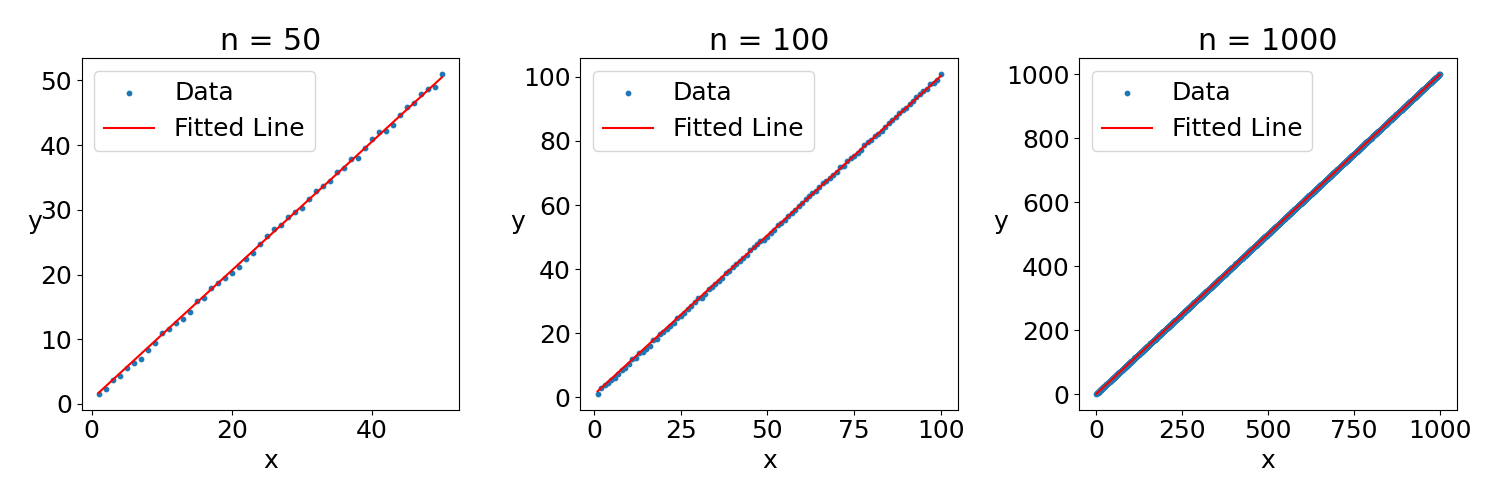
\includegraphics[width=0.99\columnwidth]{figures/lin.png}
        \caption{PGD for different learning rates and domains}
        \label{fig:lin}
    \end{figure}

Lastly, we can see the results for different optimizers and numbers of data points in Table~\ref{tab:performance}.
We can see that for smaller datasets, the Newton and quasi-Newton methods dominate, while 
for larger datasets the SGD is by far the quickest, with the normal gradient descent being the slowest.
Note that here we set the learning rate to be: 
$\frac{1}{n^2}$, since the gradients are a summation, and are therefore larger with more points, and this 
formula proved to work nicely.

    \begin{table}[ht]
        \centering
        \begin{tabular}{|c|c|c|c|}
        \hline
        \textbf{n} & \textbf{Method} & \textbf{Iterations} & \textbf{Time (s)} \\
        \hline
        \multirow{5}{*}{\textbf{n = 50}} & GD    & 6769  & 0.2575 \\
                                         & SGD   & 351   & 0.0027 \\
                                         & Newton& 1     & 0.0002 \\
                                         & BFGS  & 5     & 0.0002 \\
                                         & LBFGS & 7     & 0.0003 \\
        \hline
        \multirow{5}{*}{\textbf{n = 100}} & GD    & 11    & 0.0004 \\
                                         & SGD   & 223   & 0.0018 \\
                                         & Newton& 1     & 0.0002 \\
                                         & BFGS  & 3     & 0.0001 \\
                                         & LBFGS & 7     & 0.0004 \\
        \hline
        \multirow{5}{*}{\textbf{n = 1000}} & GD    & 10    & 0.0005 \\
                                         & SGD   & 25    & 0.0002 \\
                                         & Newton& 1     & 0.0002 \\
                                         & BFGS  & 5     & 0.0003 \\
                                         & LBFGS & 3     & 0.0001 \\
        \hline
        \multirow{5}{*}{\textbf{n = 10000}} & GD    & 10    & 0.0013 \\
                                         & SGD   & 12    & 0.0001 \\
                                         & Newton& 1     & 0.0005 \\
                                         & BFGS  & 3     & 0.0003 \\
                                         & LBFGS & 3     & 0.0002 \\
        \hline
        \multirow{5}{*}{\textbf{n = 100000}} & GD    & 10    & 0.0084 \\
                                         & SGD   & 6     & 0.0001 \\
                                         & Newton& 1     & 0.0026 \\
                                         & BFGS  & 6     & 0.0026 \\
                                         & LBFGS & 3     & 0.0012 \\
        \hline
        \multirow{5}{*}{\textbf{n = 1000000}} & GD    & 10    & 0.4266 \\
                                         & SGD   & 5     & 0.0001 \\
                                         & Newton& 1     & 0.0945 \\
                                         & BFGS  & 4     & 0.0892 \\
                                         & LBFGS & 4     & 0.0885 \\
        \hline
        \end{tabular}
        \vspace{3pt}
        \caption{Performance of Different Optimization Methods for the linear regression task}
        \label{tab:performance}
        \end{table}
      


        

\end{document}
